\section{Case study}
\label{sec:case_study}
In this section, we give a simple example of a co-simulation whose correct initialization demands the solution to an algebraic loop.

We consider a co-simulation of a quarter car model \cite[Section 6.4]{Schramm2014}, illustrated in \cref{fig:quarter_car}.
We omit the equations that each FMU is solving but note that gravity acts on both wheel and chassis masses and that the origin of each mass is when the springs are not displaced.
The equations and simulation model for this example are available online\footnote{\url{https://github.com/SimplisticCode/QuarterCarCaseStudy}}. 

\begin{figure}[htb]
    \centering
    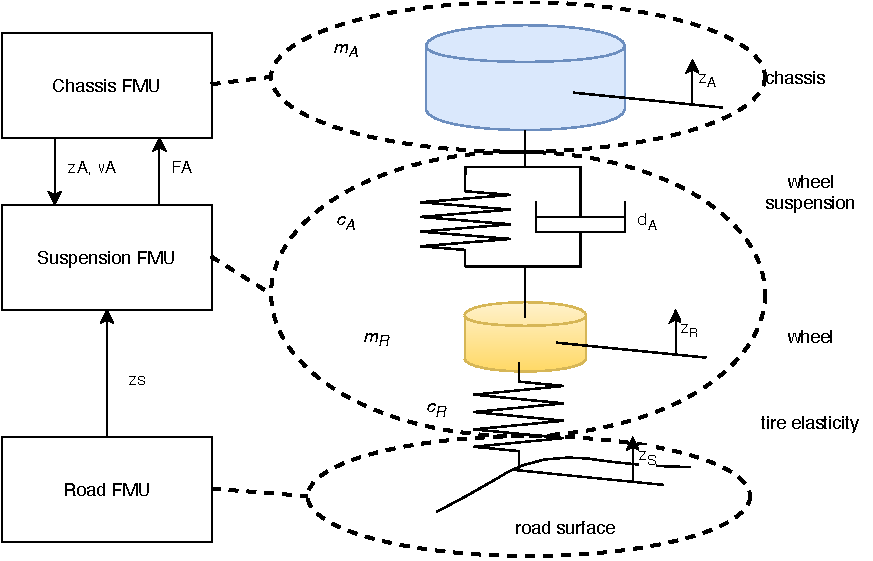
\includegraphics[width=0.8\textwidth]{images/quarter_car.pdf}
    \caption{Quarter car model co-simulation. Adapted from \cite[Section 6.4]{Schramm2014}.}
    \label{fig:quarter_car}
\end{figure}

The FMUs need initial conditions specified by equations that restrict the possible initial values for the position and velocity of the wheel and chassis masses.
\Cref{fig:init_state_0_sim} illustrates what happens when we simply set those positions and velocities to zero.
Note that, because of gravity, the car chassis bounces on the suspension wheel, with a maximum compression of about 17cm. This is most likely an invalid scenario, as the suspension of the car might not be rated to be displaced that much. In any case, the purpose of simulation studies involving quarter car models is to understand how well a suspension system absorbs shock when the car goes over a bump, not when the car is \emph{falls on the road}, which is what the simulation results in \cref{fig:init_state_0_sim} resemble.

\begin{figure}[htb]
\centering
\begin{tikzpicture}
    \begin{axis}[
        at={(0,0)},
        width= 12cm,
        height = 8cm,
        ymin=-0.2,
        ymax=0.05,
        xmin=0,
        xmax=4.1,
        grid=both,
        grid style={line width=.1pt, draw=gray!10},
        major grid style={line width=.2pt,draw=gray!50},
        axis lines=middle,
        minor tick num =5,
        axis line style={latex-latex},
        ticklabel style={font=\tiny,fill=white},
        minor tick style={draw=none},
        minor grid style={thin,color=black!10},
        ylabel= Car position,
        xlabel= Time (s),
        tick align=outside,
        x label style={at={(axis description cs:0.5,-0.1)},anchor=north},
        y label style={at={(axis description cs:-0.1,.5)},rotate=90,anchor=south},
        xlabel style={color=blue!50!cyan},
        ylabel style={align=center,rotate=-90,color=blue!50!cyan},
        x tick label style={
            /pgf/number format/assume math mode, font=\sf\scriptsize}
        ]
    \addplot [line width=2.5pt, red] table [x=a, y=b, col sep=comma] {incorrect.csv};
\end{axis}
\end{tikzpicture}
    \caption{Simulation results when position and velocity of the chassis mass is zero.}
    \label{fig:init_state_0_sim}
\end{figure}

The correct way to initialize this co-simulation scenario is to force the master algorithm to calculate the valid initial velocities and position from equations that force the accelerations and velocities on the masses to be zero.
This will force the co-simulation to initialize to a steady state.

To make the above explanation concrete, we now show the equations that are active at the initial time for each FMU for a correct initialization, and we show that there is an algebraic loop.

For the road FMU, the initial equation is simply the initial height of the road surface, which in this case is zero, i.e., $z_s=0$.
For the suspension FMU, the following equations are active:
\begin{align}
& a_R = 0.0 & \text{Acceleration of tire} \\
& v_R = 0.0 & \text{Velocity of tire} \\
& F_{gR} = 9.81 * m_R  & \text{Gravity on the tire} \\
& F_R = - c_R * z_R  & \text{Rubber force acting on tire} \\
& F_A = c_A * (z_A - z_R) + d_A * (v_A - v_r)  & \text{Suspension force acting on tire} \\
& F_{\mathit{total}} = F_R + F_A - F_{gR} & \text{Total forces acting on tire} \\
& a_R = (1/m_R) * F_{\mathit{total}}  & \text{Acceleration of tire}
\end{align}
Finally, for the Chassis FMU, the following equations are active at the initial time:
\begin{align}
& a_A = 0.0 & \text{Acceleration of chassis} \\
& v_A = 0.0 & \text{Velocity of chassis} \\
& F_{gA} = 9.81 * m_A  & \text{Gravity on the chassis} \\
& a_A = (1/m_A) * (- F_A - F_{gA})  & \text{Acceleration of chassis}
\end{align}

To see that there is an algebraic loop, note that the output $z_A$ of the chassis FMU is not restricted directly, but instead has to be computed from the acceleration equations $a_A = 0 = (1/m_A) * (- F_A - F_{gA})$.
The later contains the output $F_A$ of the Suspension FMU.
This output, in turn, depends on $z_A$, thus yielding an algebraic loop.
\Cref{fig:init_state_correct_sim} shows the simulation results when the algebraic loop is properly solved during initialization.

\begin{figure}[htb]
\centering
\begin{tikzpicture}
    \begin{axis}[
        %at={(0,0)},
        width= 12cm,
        height = 8cm,
        ymin=-0.18,
        ymax=-0.05,
        xmin=0,
        xmax=4.1,
        grid=both,
        grid style={line width=.1pt, draw=gray!10},
        major grid style={line width=.2pt,draw=gray!50},
        axis lines=middle,
        minor tick num =5,
        axis line style={latex-latex},
        ticklabel style={font=\tiny,fill=white},
        minor tick style={draw=none},
        minor grid style={thin,color=black!10},
        x label style={at={(axis description cs:0.5,-0.1)},anchor=north},
        y label style={at={(axis description cs:-0.1,.5)},rotate=90,anchor=south},
        ylabel= Car position,
        xlabel= Time (s),
        tick align=outside,
        xlabel style={color=blue!50!cyan},
        ylabel style={align=center,rotate=-90,color=blue!50!cyan},
        x tick label style={
            /pgf/number format/assume math mode, font=\sf\scriptsize}
            ]
    \addplot [line width=2.5pt, red] table [x=a, y=b, col sep=comma] {correct.csv};
\end{axis}
\end{tikzpicture}
    \caption{Simulation results starting from a correct initial state (a steady state).}
    \label{fig:init_state_correct_sim}
\end{figure}